%Template by Mark Jervelund - D1 - 2015 - mjerv15@student.sdu.dk

\documentclass[a4paper,10pt,titlepage]{report}

\usepackage[utf8]{inputenc}
\usepackage[T1]{fontenc}
\usepackage[english]{babel}
\usepackage{amssymb}
\usepackage{amsmath}
\usepackage{amsthm}
\usepackage{graphicx}
\usepackage{fancyhdr}
\usepackage{mathtools}
\usepackage{color}
\usepackage{lastpage}
\usepackage{listings}
\usepackage{algorithm}
\usepackage{algpseudocode}
\usepackage[document]{ragged2e}
\usepackage[margin=1in]{geometry}
\usepackage{color}
\usepackage{datenumber}
\usepackage{venndiagram}
\usepackage{chngcntr}
\setdatetoday
\addtocounter{datenumber}{0} %date for dilierry standard is today
\setdatebynumber{\thedatenumber}
\date{}
\setcounter{secnumdepth}{0}
\pagestyle{fancy}
\fancyhf{}

\newcommand{\Z}{\mathbb{Z}}
\lhead{Computer Architecture (DM548))}
\rhead{Mark Jervelund (Mjerv15)}
\rfoot{Page  \thepage \, of \pageref{LastPage}}
\counterwithin*{equation}{section}

\begin{document}
\begin{titlepage}
\centering
    \vspace*{9\baselineskip}
    \huge
    \bfseries
    Title \\
    
    \normalfont 
	\huge    
    Notes (DM549)  \\[4\baselineskip]
    \normalfont
	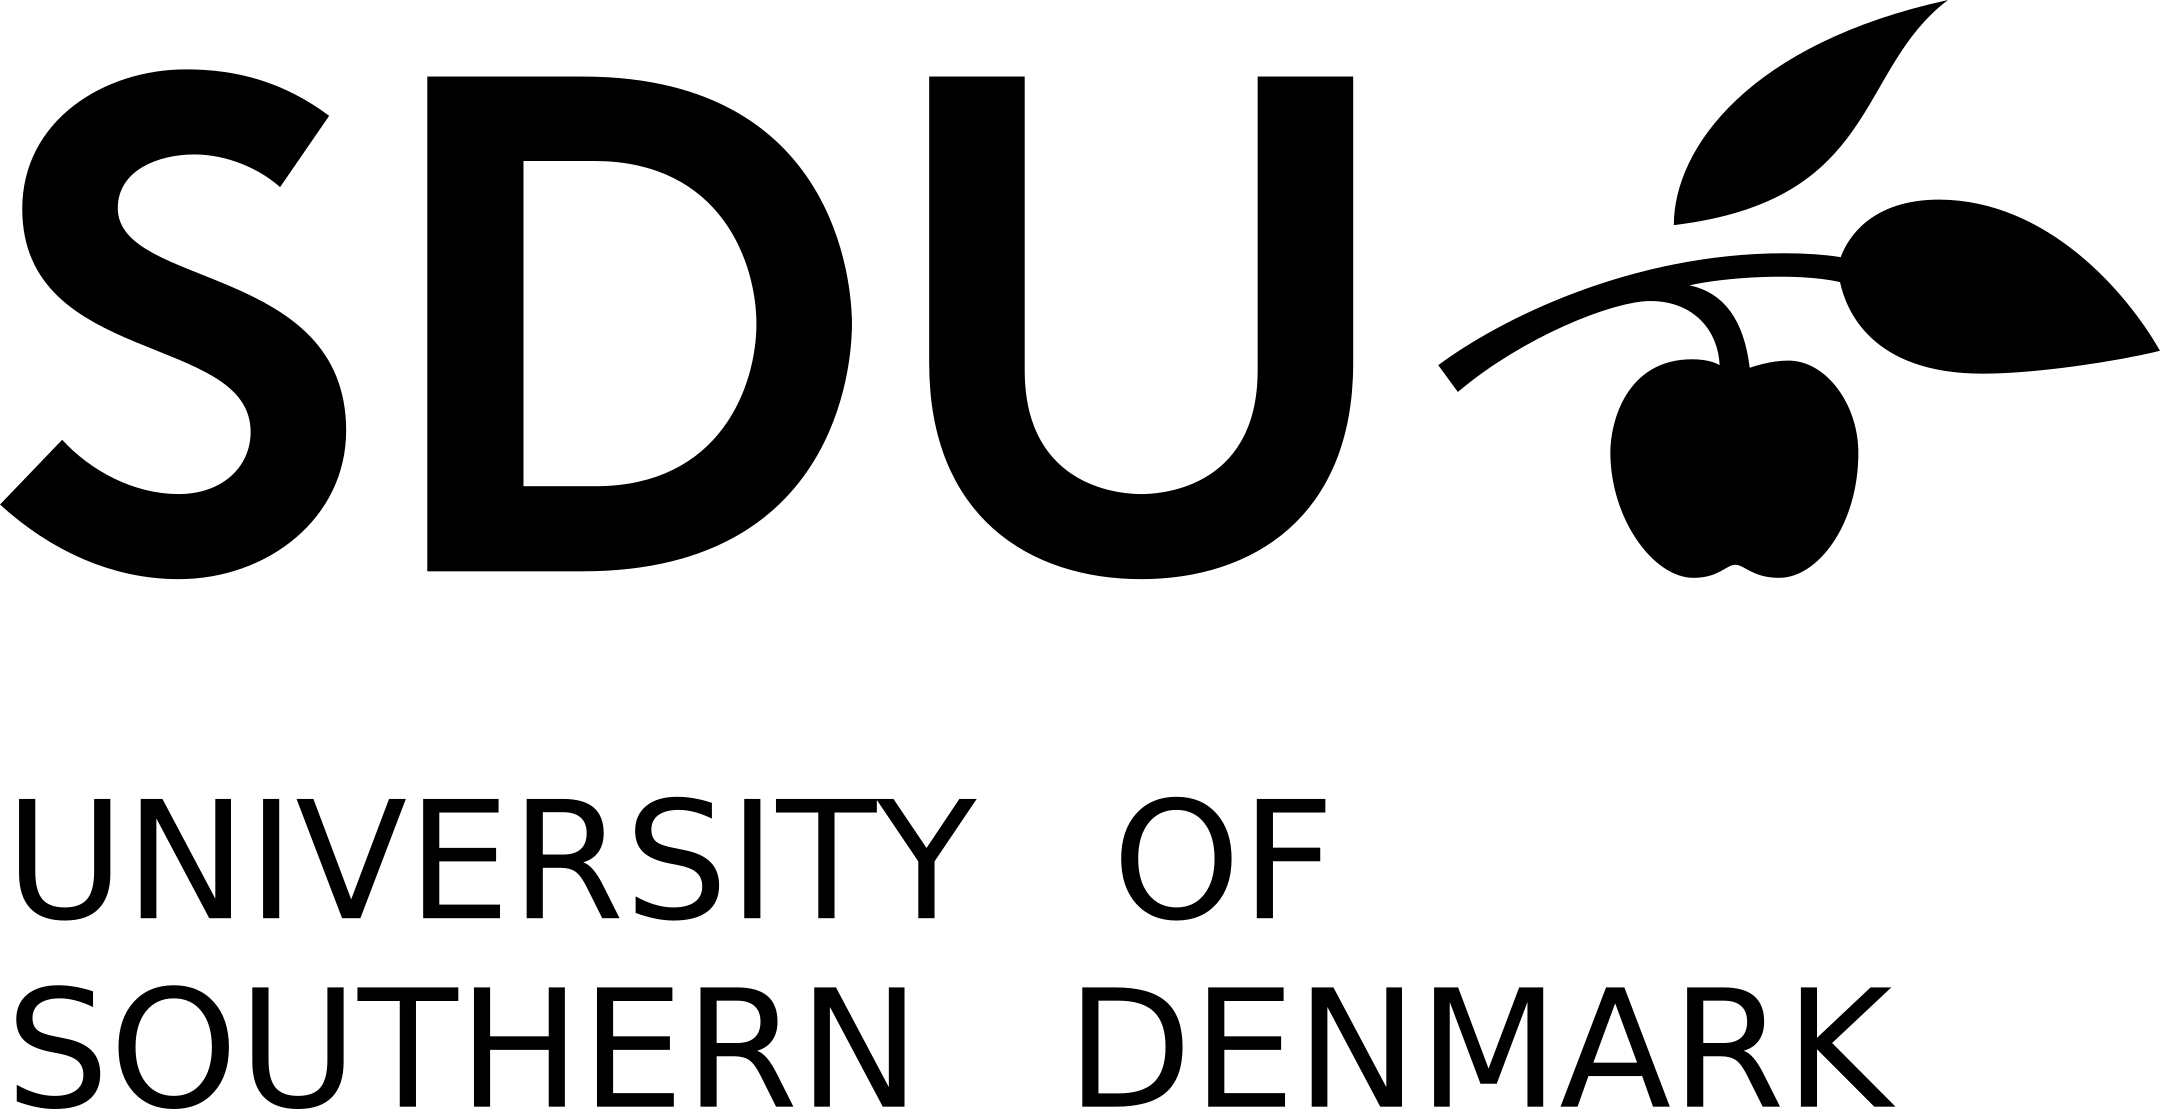
\includegraphics[scale=1.5]{SDU_Logo}
    \vfill\ 
    \vspace{5mm}
    IMADA \\
    \vspace{5mm} 
    Mark Jervelund - Mjerv15
    \\
    %Uffe Thorsen - math
    %Kristine Vitting Klinkby Knudsen - Datalogi
    %Martin Østergaard Villumsen - prog
    %Uffe Thorsen \\ \vspace{5mm}
    \textbf{\datedate}  \bf{} \\[2\baselineskip]
\end{titlepage}

%\renewcommand{\thepage}{\roman{page}}% Roman numerals for page counter
%\tableofcontents

%\newpage
\setcounter{page}{1}
\renewcommand{\thepage}{\arabic{page}}
\section{Task Design}
$
Set \ A = \emptyset 
$
\\
$
A \mapsto B
$
\\
$
\alpha
$
\\
$
\mathbb{R} \mathbb{C} \mathbb{I} \mathbb{N}
$
\\
$
\mid
$
\begin{equation}

\end{equation}
\begin{bmatrix}
  1 & 1 & 1 & = & 6 \\
  2 & 4 & 1 & = & 5 \\
  0 & -1 & 0 & = & 1 
\end{bmatrix} 
\xRightarrow[\text{}]{\text{r2 = R2 - 2R1}}
\begin{bmatrix}
  1 & 1 & 1 & = & 6 \\
  0 & 2 & -1 & = & 5-12 \\
  0 & -1 & 0 & = & 1 
\end{bmatrix} 
\xRightarrow[\text{Beloe}]{\text{Above}}
\begin{bmatrix}
  1 & 1 & 1 & = & 6 \\
  0 & 2 & -1 & = & -7 \\
  0 & 0 & 1/2 & = & -5/2 
\end{bmatrix}
\end{equation}
\begin{equation}
  \begin{cases}
    2x_2 -5 = 7\\
    2x_1 + 4x_2 + x_3 = 3 \\
    1/2 x_3 = -5/2 = x_3 = 5
  \end{cases}
\end{equation}
\colorlet{80black20white}{black!75}
\colorbox{80black20white}{test}

\newpage
\section{Lecture notes}



\newpage
\section{Feb}
\subsection{ex1 - page 1}
a)
\\
b)
\\
c)
\\
d)
\\
e)
\\
f)
\\
g)
\\
h)
\\
i
\\
j)
\\
k)
\\
\subsection{ex1 - page 2}




\subsection{ex2}
Vectors
\\
$
\begin{matrix}
  A = { 
\begin{bmatrix}
  1 & 3 & 5 \\
  -1 & 1 & 0
 \end{bmatrix}
 } & B = { 
\begin{bmatrix}
  1 & 0 & 1 \\
  2 & 1 & 1 \\
  1 & 1 & -1
 \end{bmatrix}
 } \\
  C = { 
\begin{bmatrix}
  1 & 1 \\
  3 & 2 \\
  -1 & 4
 \end{bmatrix}
 } & d = { 
\begin{bmatrix}
  2  \\
  -1 \\
  1
 \end{bmatrix}
 }
 \end{matrix}
 $
\\
a)
\\
Ad
\\
b)
\\
AB+C
\\
c)
\\
A+Ct
\\
d)
\\
$
CtC = { 
\begin{bmatrix}
  1*1+3*3+(-1)*1 & 1*1+3*2+(-1)*4 \\
  2 & -4
 \end{bmatrix}
 } =
 { 
\begin{bmatrix}
  9 & 3 \\
  2 & -4
 \end{bmatrix}
 }
$
\\
e)
\\ Not done 
\\
$
BC = { 
\begin{bmatrix}
  1*1+3*3+(-1)*1 & 1*1+3*2+(-1)*4 \\
  2 & -4
 \end{bmatrix}
 } =
$
\\
f)
\\
dtB
\\
g)
\\
Cd
\\
h)
\\
$
dtd = { 
\begin{bmatrix}
  2*2+ 1+1
 \end{bmatrix}
 } = 6
$
\\
i)
\\
$
ddt = { 
\begin{bmatrix}
  2*2 & -2 & 2 \\
  2*(-1) & (-1)*(-1) & -1 \\
  2 & -1 & 1
 \end{bmatrix}
 } = 
 { 
\begin{bmatrix}
  4 & -2 & 2 \\
  (-2) & 1 & -1 \\
  2 & -1 & 1
 \end{bmatrix}
 }
$
\\
j)
\\
A/C
\\
k)
\\
C/A
\subsection{Sheet4}

\subsection{exercise 1}
%$\overrightarrow{m}$ $\dot$ $\overrightarrow{v}$ = $\overrightarrow{m}$ $^t$ $\overrightarrow{v}$ 
I = indentity matrix.

$vec \dot vec = m + m-1 = 2m-1$\\
$Y = ABx = $\\
$Matrix \dot vec = M(2m-1)= 2m^2$
$Y = (AB)x = m^3 + 2m^2$ \\
$Matrix \dot Matrix = mp(2m-1 = 2m^3$
$Y = A(Bx) = 2m^2+2m^2$\\

uvx are vectors
$A = I + uv^t = m^2+m^2+2m^2 = nm^2$\\
$y = Ax =  $\\

$w = I + (v^tx)u = 2m-1+m+m = nm+1 $\\

$y = x+w =  $\\

\subsection{exercise 2}

Planespeed1 = 1365 / 3 = 445
planespeed2 = 870 / 2 = 435

Speeddif = 10 so wind is = 5 mph

\subsection{exercise 3}

1)\\
$8* 0.32 = x 1/2 + y 1/10 $\
2)\\
$8 = x+y$\\
3)\\
$x = 8 - y$\\
4)\\
$8*0.32 = (8-y)+1/2+y*1/10 $\\


\subsection{exercise 4}
\begin{equation}
  \begin{cases}
    x_1 + x_2 + x_3 = 6\\
    2x_1 + 4x_2 + x_3 = 3 \\
    2x_1 + 3x_2 + x_3 = ?
  \end{cases}
\end{equation}
\begin{equation}
\begin{bmatrix}
  1 & 1 & 1 & = & 6 \\
  2 & 4 & 1 & = & 5 \\
  2 & 3 & 1 & = & 6 
\end{bmatrix} => 
\begin{bmatrix}
  1 & 0 & 0 & = & 6 \\
  0 & 1 & 0 & = & 5 \\
  0 & 0 & 1 & = & 6 
\end{bmatrix}
\end{equation}


\begin{equation}
\begin{bmatrix}
  1 & 1 & 1 & = & 6 \\
  2 & 4 & 1 & = & 5 \\
  0 & -1 & 0 & = & 1 
\end{bmatrix} 
\xRightarrow[\text{}]{\text{r2 = R2 - 2R1}}
\begin{bmatrix}
  1 & 1 & 1 & = & 6 \\
  0 & 2 & -1 & = & 5-12 \\
  0 & -1 & 0 & = & 1 
\end{bmatrix} 
\xRightarrow[\text{}]{\text{R3 = R3 + 1/2 R2}}
\begin{bmatrix}
  1 & 1 & 1 & = & 6 \\
  0 & 2 & -1 & = & -7 \\
  0 & 0 & 1/2 & = & -5/2 
\end{bmatrix}
\end{equation}

\begin{equation}
  \begin{cases}
    2x_2 -5 = 7\\
    2x_1 + 4x_2 + x_3 = 3 \\
    1/2 x_3 = -5/2 = x_3 = 5
  \end{cases}
\end{equation}











\end{document}
